%% IROS 2027 format (IEEE RAS conference template, ieeeconf.cls from PaperPlaza).
%% Build:  tectonic report_iros.tex      (or pdflatex twice)
\documentclass[letterpaper, 10 pt, conference]{ieeeconf}

\IEEEoverridecommandlockouts
\overrideIEEEmargins

\usepackage{iftex}
\ifXeTeX  % Tectonic/XeLaTeX: Times via TeX Gyre Termes; pdflatex (Overleaf): times
  \usepackage{fontspec}
  \setmainfont{texgyretermes}[Extension=.otf, UprightFont=*-regular,
    BoldFont=*-bold, ItalicFont=*-italic, BoldItalicFont=*-bolditalic]
\else
  \usepackage{times}
\fi
\usepackage{amsmath,amssymb}
\usepackage{graphicx}
\usepackage{booktabs}
\usepackage{multirow}
\usepackage{url}
\usepackage{xcolor}
\usepackage{tikz}
\usetikzlibrary{positioning,arrows.meta,fit}

\newcommand{\nopath}{\texttt{NO\_PATH}}
\newcommand{\Lt}{\mathrm{LTL}_f}

\title{\LARGE \bf
Intent Forms, Not Formulas: Natural-Language Path Planning\\
with Guaranteed Walkable Paths
}

\author{Shashi Bhidodiya$^{1}$ and Krishna Kumayu$^{1}$% <-this % stops a space
\thanks{$^{1}$Shashi Bhidodiya and Krishna Kumayu are B.Tech.\ students in the
        Department of Computer Science and Engineering, Indian Institute of
        Technology Kanpur, Uttar Pradesh - 208016, India
        \mbox{\tt\small \{shashib23, kkrishna23\}@iitk.ac.in}}%
}

\begin{document}

\maketitle
\thispagestyle{empty}
\pagestyle{empty}

%%%%%%%%%%%%%%%%%%%%%%%%%%%%%%%%%%%%%%%%%%%%%%%%%%%%%%%%%%%%%%%%%%%%%%%%%%%%%%%%
\begin{abstract}
People give navigation instructions that mix a destination, prohibitions, ordered
stops and soft preferences: \emph{``go to the lab, don't go through the workshop,
stop at the store room first, and stay in the corridor if you can.''} Asking a large
language model (LLM) for the path accepts any phrasing but guarantees nothing;
translating the sentence into temporal logic gives guarantees but the formula is hard
to get right and cannot express ``if you can.'' We separate the two jobs. The LLM sees
only the instruction and the region names and fills a small, readable \emph{intent
form}; it never sees the map or emits a coordinate. The form is validated, compiled
into walls and cell weights, and solved by A* over (cell, waypoint-progress) states,
and an independent verifier checks every path. We prove that every returned path is
walkable even when the LLM misreads the instruction, and that, given a correct parse,
it satisfies all hard constraints, is optimal, is never missed when one exists, and
lengthens by at most a fixed factor because of soft preferences. On a benchmark of 495
instructions over 20 floor plans, using the same LLM for every method, our method is
correct on 100\% of inputs, an LLM$\to\Lt\to$automaton planner on 88\% (61\% on
ordered stops), and an end-to-end LLM planner produces a walkable path in 1 of 161
attempts.
\end{abstract}

%%%%%%%%%%%%%%%%%%%%%%%%%%%%%%%%%%%%%%%%%%%%%%%%%%%%%%%%%%%%%%%%%%%%%%%%%%%%%%%%
\section{Introduction}

A grid planner such as A* \cite{hart1968} takes one goal cell. A person instructing a
robot gives much more: a destination, places that must not be entered, places to
visit in a given order, and preferences that should be honoured only when they are
cheap. Two families of methods turn such language into robot behaviour, and each
falls short in a different way.

\emph{LLMs as planners.} An LLM can read the map (as text) and write the path
directly \cite{aghzal2023ppnl}, or propose waypoints that a search
connects \cite{meng2024llmastar}. This accepts any phrasing, but nothing guarantees that
the path avoids walls or forbidden rooms, and LLMs are known to be unreliable at
multi-step planning \cite{valmeekam2023,kambhampati2024}.

\emph{LLMs as translators to formal logic.} The sentence is translated into a
temporal-logic formula, which an automaton-based planner then satisfies
\cite{liu2023lang2ltl,fuggitti2023nl2ltl,cosler2023nl2spec,chen2024autotamp}. Given the
right formula, the plan is correct by construction \cite{kressgazit2009}. In practice
the formula is the weak point: it is hard to write correctly, it is unreadable to the
user who must check it, and a Boolean formula cannot express ``if you can.''

We take a middle path in the spirit of LLM+P \cite{liu2023llmp} and LLM-modulo
planning \cite{kambhampati2024}: \textbf{the LLM decides \emph{what} the user wants; A*
decides \emph{how}.} The LLM fills a fixed, five-field intent form; everything
downstream is classical and verified. Our contributions are:

\begin{enumerate}
\item A pipeline in which LLM output can influence the path \emph{only} through a
  validated intent form, with a product-graph A* that handles prohibitions, strictly
  ordered waypoints and weighted soft preferences in one optimal search (Sec.~\ref{sec:method}).
\item Six guarantees with short proofs: walkability independent of the parse (T1),
  soundness, completeness and optimality given the parse (T2--T4), a bounded detour
  for soft preferences (T5), and exact correspondence of the hard part with an $\Lt$
  formula (T6) (Sec.~\ref{sec:theory}).
\item A benchmark of 165 instructions $\times$ 3 wordings with gold intent forms, gold
  $\Lt$ formulas and solver-verified labels, and a controlled comparison with an
  end-to-end LLM planner and an LLM$\to\Lt$ planner using the same LLM, prompt
  budget and maps (Sec.~\ref{sec:eval}).
\end{enumerate}

%%%%%%%%%%%%%%%%%%%%%%%%%%%%%%%%%%%%%%%%%%%%%%%%%%%%%%%%%%%%%%%%%%%%%%%%%%%%%%%%
\section{Related Work}

\textbf{Language grounding for navigation.} Early work grounded commands with
probabilistic graphical models over spatial relations \cite{tellex2011}. LLM-based
systems now select skills \cite{ahn2022saycan}, write robot programs
\cite{liang2023cap,singh2023progprompt}, or plan in text. None of these give
guarantees on the geometric path.

\textbf{LLMs as path planners.} PPNL \cite{aghzal2023ppnl} benchmarks LLMs that read a
grid and output a path, and finds frequent invalid moves on larger grids; our M1
baseline follows this setting. LLM-A* \cite{meng2024llmastar} lets the LLM propose
intermediate waypoints that A* connects, improving efficiency; the path is walkable,
but the LLM still reasons about coordinates and constraints such as prohibitions or
ordering are not guaranteed.

\textbf{LLMs as translators to temporal logic.} Lang2LTL \cite{liu2023lang2ltl},
NL2LTL \cite{fuggitti2023nl2ltl}, nl2spec \cite{cosler2023nl2spec} and AutoTAMP
\cite{chen2024autotamp} translate language into LTL or signal temporal logic, which is
then planned against with automata-based methods \cite{kressgazit2009,smith2011}. Our
M2 baseline follows this route with finite-trace LTL ($\Lt$) \cite{degiacomo2013} and
Spot \cite{duretlutz2022}. We show that, on the hard constraints, our intent form is
exactly a fragment of $\Lt$ (T6), so the comparison isolates the effect of the
\emph{target representation} the LLM must produce.

\textbf{LLMs with classical planners.} LLM+P \cite{liu2023llmp} has the LLM write a PDDL
problem for a classical planner, and the LLM-modulo view \cite{kambhampati2024}
argues for LLMs paired with sound external verifiers. Our work applies this idea to
geometric navigation with soft preferences, with proofs specific to the grid setting.

%%%%%%%%%%%%%%%%%%%%%%%%%%%%%%%%%%%%%%%%%%%%%%%%%%%%%%%%%%%%%%%%%%%%%%%%%%%%%%%%
\section{Problem Setting}

\textbf{Map.} An 8-connected grid; $F$ is the set of free cells. Each free cell belongs
to at most one named region (rooms, a corridor); $R_r$ is the set of cells of region $r$.
A diagonal step is legal only if both orthogonal neighbours are also allowed (no corner
cutting). Step length $d(v,u)$ is $1$ or $\sqrt2$.

\textbf{Intent form.} $I = (g, X, (w_1,\dots,w_m), P, A)$: a goal region $g$, forbidden
regions $X$, ordered waypoints $w_j$, preferred regions $P$ and avoided regions $A$.
The \emph{sequence} is $u_1,\dots,u_{m+1} = w_1,\dots,w_m,g$. $I$ is \emph{well-formed}
if all names exist on the map, the sequence has no repeats, no sequence element is
forbidden, and $P \cap A = \emptyset$.

\textbf{Satisfaction.} Let $S_I = F \setminus \bigcup_{x\in X} R_x$. Forbidden cells are
treated as walls, also for the corner rule, so a path never grazes them. Let $e_j(\pi)$ be
the first index at which path $\pi$ enters $u_j$. A path $\pi$ from start $s$
\emph{satisfies} $I$ if it is valid in $S_I$, ends in $g$, enters every $u_j$, and
$e_1 < e_2 < \dots < e_{m+1}$ (\emph{strict ordering}: ``A before B'' means B is never
entered before A).

\textbf{Cost.} Cell weight $w(u) = 0.5$ if preferred, $3$ if avoided, else $1$; path
cost $J(\pi) = \sum_i d(v_i,v_{i+1})\,w(v_{i+1})$ and length
$L(\pi) = \sum_i d(v_i,v_{i+1})$. The task is to return a minimum-cost satisfying path,
or \nopath{} if none exists.

%%%%%%%%%%%%%%%%%%%%%%%%%%%%%%%%%%%%%%%%%%%%%%%%%%%%%%%%%%%%%%%%%%%%%%%%%%%%%%%%
\section{Method}
\label{sec:method}

\begin{figure}[t]
\centering
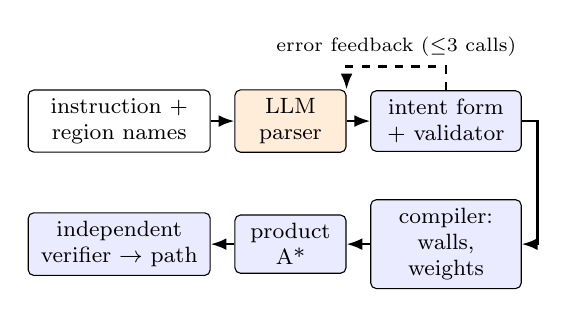
\begin{tikzpicture}[
  box/.style={draw, rounded corners=2pt, align=center, font=\footnotesize,
              minimum height=7mm, inner sep=3pt},
  llm/.style={box, fill=orange!15},
  cls/.style={box, fill=blue!8},
  arr/.style={-{Latex[length=2mm]}, thick},
  node distance=4mm and 3mm]
\node[box, text width=21mm] (in) {instruction +\\region names};
\node[llm, right=of in, text width=12mm] (llm) {LLM\\parser};
\node[cls, right=of llm, text width=17mm] (val) {intent form\\+ validator};
\node[cls, below=6mm of val, text width=17mm] (cmp) {compiler:\\walls, weights};
\node[cls, left=of cmp, text width=12mm] (pa) {product\\A*};
\node[cls, left=of pa, text width=21mm] (ver) {independent\\verifier $\to$ path};
\draw[arr] (in) -- (llm);
\draw[arr] (llm) -- (val);
\draw[arr] (val.east) -- ++(2mm,0) |- node[pos=0.25,right,font=\scriptsize]{} (cmp.east);
\draw[arr] (cmp) -- (pa);
\draw[arr] (pa) -- (ver);
\draw[arr, dashed] (val.north) -- ++(0,3mm) -| node[pos=0.25,above,font=\scriptsize]{error feedback ($\le$3 calls)} (llm.north east);
\end{tikzpicture}
\caption{Pipeline (M3). Orange: the only learned component; it sees the instruction and
region names, never the map, and outputs a five-field intent form. Blue: classical,
verified components.}
\label{fig:pipeline}
\end{figure}

Fig.~\ref{fig:pipeline} shows the pipeline.

\textbf{Parser.} The LLM receives the instruction, the list of region names and two
worked examples, and returns JSON, e.g.
\begin{center}
\footnotesize
\texttt{\{goal: lab, forbidden: [workshop],}\\
\texttt{\ waypoints: [store\_room], prefer: [corridor], avoid: []\}}
\end{center}
The form is validated against the well-formedness rules; on failure the error is fed
back, for at most three calls. The LLM never sees the grid.

\textbf{Compiler.} Forbidden regions become walls; preferred cells get weight 0.5,
avoided cells 3, others 1.

\textbf{Product-graph A*.} A state is $(v,k)$: cell $v$ after entering the first $k$
sequence elements in order. From $(v,k)$ any legal step in $S_I$ to $u$ is allowed
\emph{unless} $u$ lies in an element not yet due, $u_{k+2},\dots,u_{m+1}$; entering
$u_{k+1}$ increments $k$. Goal states are $(v,m+1)$ with $v\in R_g$; step cost is
$d(v,u)\,w(u)$. The heuristic is $h(v) = w_{\min}\cdot \mathrm{oct}(v,R_g)$, the octile
distance to the nearest goal cell scaled by the smallest weight of any allowed cell.
The scaling is essential: with preferred cells at weight 0.5, unscaled octile
distance overestimates and A* can return a suboptimal path. A start inside a forbidden
region or inside a later sequence element returns \nopath{} with a reason.

\textbf{Verifier.} A separate module, sharing no code with the planner, re-checks
every returned path (legal moves, no forbidden cell, strict order, ends in goal) and
recomputes its cost. A failure raises an exception; it is never returned silently.

%%%%%%%%%%%%%%%%%%%%%%%%%%%%%%%%%%%%%%%%%%%%%%%%%%%%%%%%%%%%%%%%%%%%%%%%%%%%%%%%
\section{Guarantees}
\label{sec:theory}

We state the results; full proofs are in the project repository. Two facts drive
them. \emph{(F1)} $h$ is consistent: octile distance obeys the triangle inequality and
every step costs at least $w_{\min}\,d(v,u)$. \emph{(F2)} The counter is honest and
complete: along any planner path $k$ counts the elements entered, in order; and every
satisfying path, annotated with this count, is a planner path of the same cost.

\textbf{T1 (walkability, unconditional).} For every well-formed intent form, even one
that misreads the instruction, the output is \nopath{} or a physically valid path.
\emph{Proof:} every planner step is legal in $S_I\subseteq F$. The LLM can only remove
cells, change positive weights, or choose regions to visit; none adds a step through a
wall. \hfill$\square$

\textbf{T2--T4 (soundness, completeness, optimality).} Every returned path satisfies $I$;
\nopath{} is returned only if no satisfying path exists; and the returned path has
minimum cost $J$. \emph{Proof:} T2 from F2. T3: by F2 a goal state is reachable, and
the state space is finite. T4: A* with a consistent heuristic and positive costs is
optimal \cite{hart1968}, and by F2 no satisfying path is cheaper. \hfill$\square$

\textbf{T5 (bounded detour).} Let $L^*$ be the shortest length of a path satisfying
the hard part of $I$. Then
$L(\hat\pi) \le \tfrac{w_{\max}}{w_{\min}} L^* \le 6L^*$; with preferences only,
$\le 2L^*$. \emph{Proof:} preferences change only weights, so the satisfying paths are
the same; $w_{\min}L(\hat\pi) \le J(\hat\pi) \le J(\pi_{L^*}) \le w_{\max}L^*$ by
T4. \hfill$\square$

T5 is the formal content of ``if you can'': a preference can never cause an unbounded
detour and never changes whether a path exists.

\textbf{T6 ($\Lt$ correspondence).} Define
$\psi_{m+1} = \mathbf{F}(g \wedge \mathit{last})$,
$\psi_j = \neg(u_{j+1}\vee\dots\vee u_{m+1})\,\mathbf{U}\,(u_j \wedge \psi_{j+1})$ and
$\varphi_I = \mathbf{G}\,\neg\bigvee_{x\in X} x \wedge \psi_1$.
On a \emph{corner-separated} map (no physically legal diagonal step grazes a region
without entering it), a valid path satisfies the hard part of $I$ iff its trace of
region labels satisfies $\varphi_I$. All our maps are corner-separated (checked
automatically). T6 provides the gold formulas for the benchmark and shows that, on
hard constraints, the intent form and the $\Lt$ route have the same expressive power
on our instructions; differences between M2 and M3 are therefore due to translation.

\textbf{From proofs to code.} Property-based tests \cite{maciver2019hypothesis} check
T1--T5 on 1000 random grids per property against an independent NetworkX
\cite{hagberg2008} product-graph solver, and in the evaluation the runtime verifier
rejected 0 of the 850 paths our pipeline returned.

%%%%%%%%%%%%%%%%%%%%%%%%%%%%%%%%%%%%%%%%%%%%%%%%%%%%%%%%%%%%%%%%%%%%%%%%%%%%%%%%
\section{Evaluation}
\label{sec:eval}

\subsection{Benchmark}

\textbf{Maps.} 20 procedurally generated $40\times40$ floor plans (6 easy, 7 medium, 7
hard) with rooms, one main corridor and 1-cell doorways, plus 10 $15\times15$ plans.
Every cell's region is known exactly.

\textbf{Instructions.} 165 instructions in six categories: plain (20), prohibition (35),
stop (30), ordering (30), soft (35) and infeasible (15); 135 are templated and 30 are
hand-written in deliberately messy phrasing. Each has three wordings (495 inputs), a
gold intent form, a gold $\Lt$ formula (from T6) and machine-checkable constraints.
Feasibility labels and optimal costs come from an independent NetworkX solver, never
from our planner. Constraints are sampled so that they matter: every prohibition
changes the optimal route, and every soft instruction is one where honouring the
preference changes the route. A further 20 instructions use the $15\times15$ maps.

\subsection{Methods}

\begin{itemize}
\item \textbf{M0} Plain A* to the goal, ignoring constraints (floor).
\item \textbf{M1} End-to-end LLM planner: the LLM sees the ASCII map and writes the
  coordinate sequence, following the PPNL setting \cite{aghzal2023ppnl}.
\item \textbf{M2} LLM$\to\Lt\to$automaton planner, following the NL-to-LTL line
  \cite{liu2023lang2ltl,fuggitti2023nl2ltl,cosler2023nl2spec}: the LLM writes an $\Lt$
  formula over region names, Spot \cite{duretlutz2022} builds a DFA, and we search the
  product of the DFA with the grid (same moves as M3).
\item \textbf{M3} Ours.
\end{itemize}
Ablations: M2-/M3-oracle (gold formula / gold intent form), M2-harden (soft ``avoid''
written as a prohibition), M3-chain (waypoints chained with separate A* searches).
M1--M3 use the same LLM (Gemini \texttt{gemini-3.5-flash-lite} \cite{gemini2023},
temperature 0), the same region-name legend and the same budget of at most three calls
with error feedback. M2 and M3 run on all three wordings; M1 on the first, as its
failure mode is walkability. All LLM answers are cached, so every number reproduces
without API access.

\textbf{Metrics.} \emph{Correct}: all hard constraints satisfied on a feasible
instruction, or \nopath{} on an infeasible one. We report Wilson 95\% intervals
\cite{wilson1927}, exact paired McNemar tests \cite{mcnemar1947}, and bootstrap
intervals for cost ratios.

\subsection{Results}

\begin{table}[t]
\centering
\caption{Correctness per category on the $40\times40$ benchmark
(M2, M3: $n=495$; M0, M1: $n=165$). Brackets: Wilson 95\% CI.}
\label{tab:main}
\setlength{\tabcolsep}{3pt}
\footnotesize
\begin{tabular}{lccccccc}
\toprule
Method & plain & proh. & stop & order & soft & infeas. & all \\
\midrule
M0 & 100 & 0 & 10 & 0 & 100 & 0 & 35 {\scriptsize[28--43]} \\
M1 & 0 & 0 & 0 & 0 & 0 & 0 & 0 {\scriptsize[0--2]} \\
M2 & 100 & 100 & 93 & 61 & 83 & 100 & 88 {\scriptsize[85--91]} \\
\textbf{M3} & \textbf{100} & \textbf{100} & \textbf{100} & \textbf{100} & \textbf{100} & \textbf{100} & \textbf{100} {\scriptsize[99--100]} \\
\midrule
M2-oracle & 100 & 100 & 100 & 100 & 100 & 100 & 100 \\
M3-oracle & 100 & 100 & 100 & 100 & 100 & 100 & 100 \\
\bottomrule
\end{tabular}
\end{table}

\begin{figure}[t]
\centering
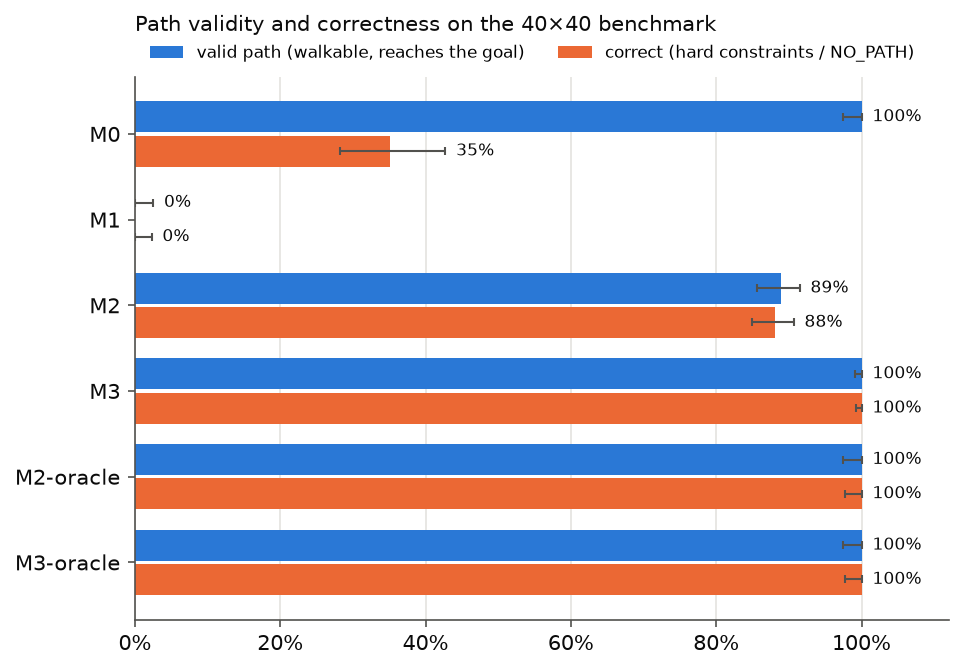
\includegraphics[width=\columnwidth]{figures/validity.png}
\caption{Valid paths on feasible instructions and overall correctness, with Wilson
95\% intervals.}
\label{fig:validity}
\end{figure}

\textbf{Overall.} Table~\ref{tab:main} and Fig.~\ref{fig:validity} summarise
correctness. M3 is correct on all 495 inputs. M2 is correct on 88\%; its losses
concentrate on ordering (61\%) and soft instructions (83\%). With gold inputs both
planners are perfect, so all of M2's loss is in translation, as T6 predicts. Paired
McNemar test, M3 vs.\ M2 on the same 495 inputs: 59 inputs only M3 got right and
0 only M2 ($p = 3.5\cdot10^{-18}$; ordering $p = 5.8\cdot10^{-11}$, soft
$p = 7.6\cdot10^{-6}$).

\begin{figure*}[t]
\centering
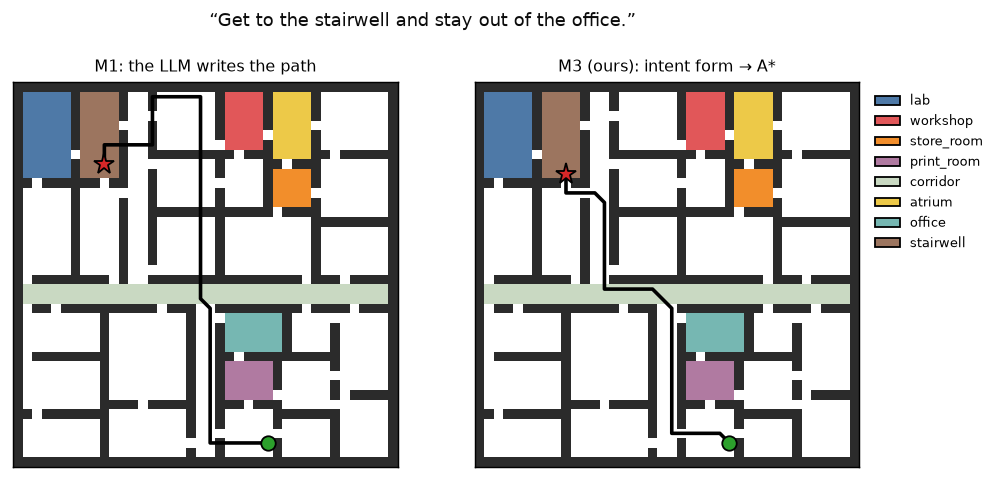
\includegraphics[width=0.62\textwidth]{figures/m1_vs_m3.png}
\caption{The same prohibition instruction. Left: the end-to-end LLM (M1) writes a path
that crosses walls. Right: M3's path, walkable by construction (T1).}
\label{fig:m1}
\end{figure*}

\textbf{End-to-end LLM planning fails on walkability.} Of M1's 161 returned paths, 160
are physically invalid (and all 20 on the $15\times15$ maps); 88\% of runs step through a
wall or forbidden cell, often jumping across the map, and on every infeasible
instruction M1 invented a path (Fig.~\ref{fig:m1}). M2 and M3 never return an invalid
path. The failure is structural, not a matter of prompt tuning: coordinate-level
output gives the model thousands of chances to make an illegal move.

\begin{table}[t]
\centering
\caption{Translation quality: intent form (M3) vs.\ $\Lt$ formula (M2).}
\label{tab:translation}
\setlength{\tabcolsep}{2pt}
\footnotesize
\begin{tabular}{lcc}
\toprule
 & M3 intent form & M2 $\Lt$ \\
\midrule
Matches gold (Spot equiv.\ for M2) & \textbf{100\%} & 56\% {\scriptsize[52--61]} \\
Same reading for all 3 wordings & \textbf{100\%} & 30\% {\scriptsize[23--37]} \\
Correct on hand-written inputs & \textbf{90/90} & 78/90 \\
No valid output in 3 calls & 0\% & 0\% \\
Mean LLM calls & 1.00 & 1.01 \\
\bottomrule
\end{tabular}
\end{table}

\textbf{Intent forms are easier to produce than formulas.} Table~\ref{tab:translation}:
the LLM's intent forms match the gold form on every input, while only 56\% of its
$\Lt$ formulas are equivalent to the gold formula, and only 30\% of instructions get
the same formula for all three wordings. M2's formulas are syntactically valid but
often semantically wrong. Many errors are harmless on the given map (157 runs were
correct despite a non-equivalent formula), but 58 changed the path. The typical
mistake on ordering is the ``next'' operator, which forces the robot to \emph{start}
in the first waypoint, e.g.\
\texttt{stairwell \& X(workshop \& X F(store\_room \& last))}, or omitting the clause
that keeps the goal unvisited before earlier waypoints.

\begin{table}[t]
\centering
\caption{Soft-preference instructions: share of path length in the preferred
corridor and in the avoided room, and length relative to M3.}
\label{tab:soft}
\setlength{\tabcolsep}{2pt}
\footnotesize
\begin{tabular}{lccc}
\toprule
Method & in preferred & in avoided & length / M3 \\
\midrule
M2-drop (ignored) & 27\% & 16\% & 0.92 \\
M2-harden (prohibited) & 27\% & 0\% & 0.96 {\scriptsize(max 1.36)} \\
M2 (LLM's encoding) & 28\% & 12\% & 0.89 \\
\textbf{M3} & \textbf{51\%} & \textbf{2\%} & 1.00 \\
\bottomrule
\end{tabular}
\end{table}

\begin{figure*}[t]
\centering
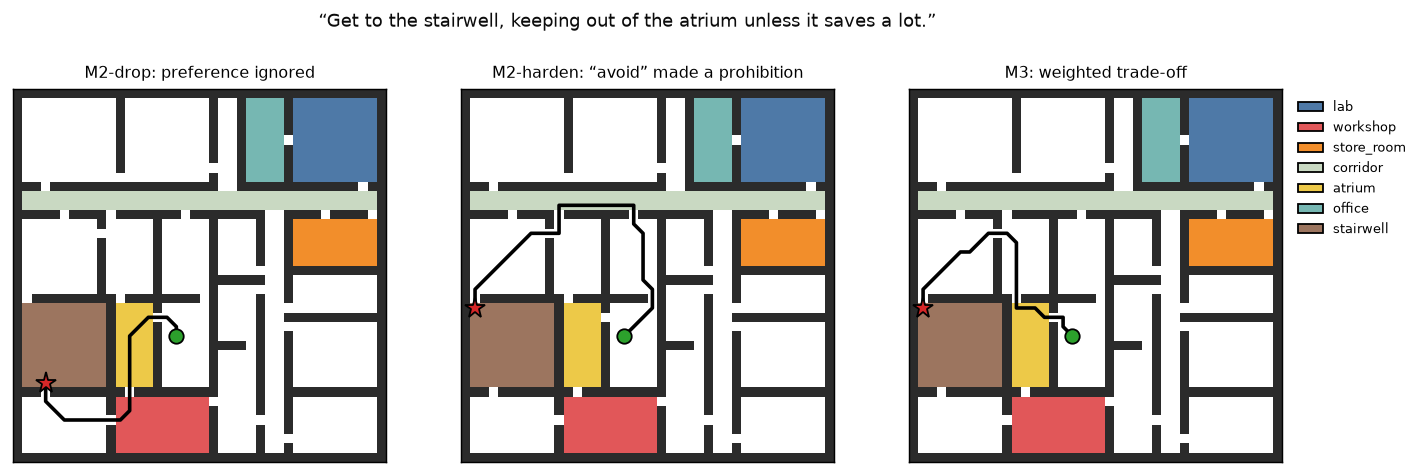
\includegraphics[width=0.85\textwidth]{figures/soft_harden.png}
\caption{A soft ``avoid'' instruction. Ignoring the preference (left) walks through the
avoided room; hardening it (middle) forces a long detour; M3 (right) trades off.}
\label{fig:soft}
\end{figure*}

\textbf{Only the intent form trades off.} A Boolean formula can only ignore a
preference or turn it into a rule. Table~\ref{tab:soft} and Fig.~\ref{fig:soft}: M3
nearly doubles the time spent in the preferred corridor and mostly stays out of
avoided rooms, at an average of 9\% extra length (maximum 23\%), far inside the T5
bound of $2\times$ for preferences (Fig.~\ref{fig:t5}). Hardening ``avoid if you can''
removes the avoided room but costs up to 36\% more length than M3 on the same
instruction.

\begin{figure}[t]
\centering
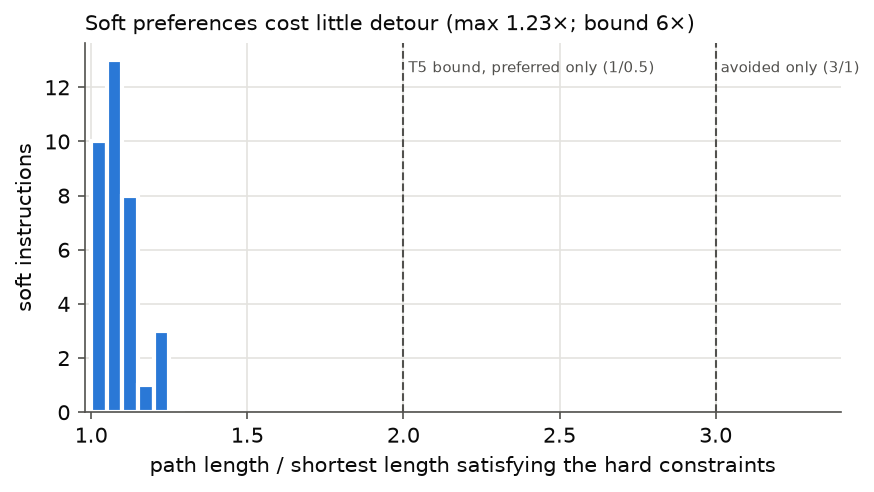
\includegraphics[width=\columnwidth]{figures/t5_detour.png}
\caption{Length of M3's soft-preference paths relative to the shortest path
satisfying the hard constraints, against the T5 bounds.}
\label{fig:t5}
\end{figure}

\textbf{Infeasibility.} On the 15 infeasible instructions (goal reachable only through a
forbidden room, or a waypoint reachable only through the goal), M2 and M3 answered
\nopath{} on every wording; by T3 this is a certificate of impossibility for the parsed
form. M1 invented a path every time; M0 ignores the constraint.

\textbf{Ablations.} M3's paths cost exactly the reference optimum (ratio 1.000); M2
plans without weights, so its correct paths cost 2.2\% more under the instruction's
preferences. Chaining waypoints with separate searches is strictly worse on 8\% of
waypoint instructions (up to 5.4\% more cost); the product search is never worse.
M3-oracle expands 744 states on average vs.\ 1{,}127 for the automaton planner, which
has no heuristic. On the $15\times15$ maps the picture is the same: M1 0\%, M2 88\%,
M3 100\%.

%%%%%%%%%%%%%%%%%%%%%%%%%%%%%%%%%%%%%%%%%%%%%%%%%%%%%%%%%%%%%%%%%%%%%%%%%%%%%%%%
\section{Limitations}

\textbf{The parser is not guaranteed.} T2--T5 hold for the parsed form; the parse
itself is measured, not proved. Our benchmark is synthetic: region names are given,
sentences are short, and most instructions are templated. Harder language will lower
M3's (and M2's) accuracy; T1 still keeps every path walkable, and errors remain visible
in a form the user can read.
\textbf{Scope of comparison.} M1 and M2 are our implementations of the
end-to-end and NL-to-LTL paradigms with a shared LLM and prompt budget, not the
original systems; we have not yet compared against hybrid planners such as LLM-A*
\cite{meng2024llmastar} or LLM+P \cite{liu2023llmp}. All results use one LLM at
temperature 0.
\textbf{Expressiveness.} The intent form covers goals, prohibitions, ordered stops and
region preferences; it does not express repetition, conditionals or metric
constraints, which full LTL can. \textbf{Abstraction.} Walkability is on an
8-connected grid without corner cutting; robot geometry and dynamics are out of scope.

%%%%%%%%%%%%%%%%%%%%%%%%%%%%%%%%%%%%%%%%%%%%%%%%%%%%%%%%%%%%%%%%%%%%%%%%%%%%%%%%
\section{Conclusion and Future Work}

Restricting the LLM to a small, validated intent form, and leaving geometry to a
verified product-graph A*, gives paths that are always walkable, provably correct
and optimal for the parsed instruction, and able to honour soft preferences with a
bounded cost. On our benchmark the LLM produced correct intent forms far more
reliably than correct temporal-logic formulas for the same instructions. Future work
is to compare against published hybrid LLM planners (LLM-A*, LLM+P) and the original
NL-to-LTL systems, to evaluate on real building maps and free-form human instructions,
to extend the form with spatial relations and repetition, and to evaluate the full
pipeline in ROS/Gazebo simulation, with a simulated mobile robot following the planned
paths, before deploying it on a real robot.

%%%%%%%%%%%%%%%%%%%%%%%%%%%%%%%%%%%%%%%%%%%%%%%%%%%%%%%%%%%%%%%%%%%%%%%%%%%%%%%%
\section*{Acknowledgment}
This work was carried out as an undergraduate project at IIT Kanpur. We thank Prof. Indranil Saha for guidance.

\begin{thebibliography}{99}
\footnotesize

\bibitem{hart1968}
P.~E. Hart, N.~J. Nilsson, and B.~Raphael, ``A formal basis for the heuristic
determination of minimum cost paths,'' \emph{IEEE Trans. Syst. Sci. Cybern.}, vol.~4,
no.~2, pp. 100--107, 1968.

\bibitem{aghzal2023ppnl}
M.~Aghzal, E.~Plaku, and Z.~Yao, ``Can large language models be good path planners?
A benchmark and investigation on spatial-temporal reasoning,'' arXiv:2310.03249, 2023.

\bibitem{meng2024llmastar}
S.~Meng, Y.~Wang, C.-F. Yang, N.~Peng, and K.-W. Chang, ``LLM-A*: Large language model
enhanced incremental heuristic search on path planning,'' in \emph{Findings of EMNLP},
2024, pp. 1087--1102.

\bibitem{valmeekam2023}
K.~Valmeekam, M.~Marquez, S.~Sreedharan, and S.~Kambhampati, ``On the planning
abilities of large language models---a critical investigation,'' in \emph{NeurIPS},
2023.

\bibitem{kambhampati2024}
S.~Kambhampati, K.~Valmeekam, L.~Guan, M.~Verma, K.~Stechly, S.~Bhambri, L.~Saldyt,
and A.~Murthy, ``Position: LLMs can't plan, but can help planning in LLM-modulo
frameworks,'' in \emph{ICML}, PMLR vol.~235, 2024, pp. 22895--22907.

\bibitem{liu2023lang2ltl}
J.~X. Liu, Z.~Yang, I.~Idrees, S.~Liang, B.~Schornstein, S.~Tellex, and A.~Shah,
``Grounding complex natural language commands for temporal tasks in unseen
environments,'' in \emph{CoRL}, PMLR vol.~229, 2023, pp. 1084--1110.

\bibitem{fuggitti2023nl2ltl}
F.~Fuggitti and T.~Chakraborti, ``NL2LTL---a Python package for converting natural
language (NL) instructions to linear temporal logic (LTL) formulas,'' in \emph{AAAI
(Demo Track)}, vol.~37, no.~13, 2023, pp. 16428--16430.

\bibitem{cosler2023nl2spec}
M.~Cosler, C.~Hahn, D.~Mendoza, F.~Schmitt, and C.~Trippel, ``nl2spec: Interactively
translating unstructured natural language to temporal logics with large language
models,'' in \emph{CAV}, LNCS vol.~13965, 2023, pp. 383--396.

\bibitem{chen2024autotamp}
Y.~Chen, J.~Arkin, C.~Dawson, Y.~Zhang, N.~Roy, and C.~Fan, ``AutoTAMP: Autoregressive
task and motion planning with LLMs as translators and checkers,'' in \emph{ICRA},
2024, pp. 6695--6702.

\bibitem{kressgazit2009}
H.~Kress-Gazit, G.~E. Fainekos, and G.~J. Pappas, ``Temporal-logic-based reactive
mission and motion planning,'' \emph{IEEE Trans. Robot.}, vol.~25, no.~6,
pp. 1370--1381, 2009.

\bibitem{liu2023llmp}
B.~Liu, Y.~Jiang, X.~Zhang, Q.~Liu, S.~Zhang, J.~Biswas, and P.~Stone, ``LLM+P:
Empowering large language models with optimal planning proficiency,''
arXiv:2304.11477, 2023.

\bibitem{tellex2011}
S.~Tellex, T.~Kollar, S.~Dickerson, M.~R. Walter, A.~G. Banerjee, S.~Teller, and
N.~Roy, ``Understanding natural language commands for robotic navigation and mobile
manipulation,'' in \emph{AAAI}, 2011, pp. 1507--1514.

\bibitem{ahn2022saycan}
M.~Ahn \emph{et al.}, ``Do as I can, not as I say: Grounding language in robotic
affordances,'' in \emph{CoRL}, PMLR vol.~205, 2022, pp. 287--318.

\bibitem{liang2023cap}
J.~Liang, W.~Huang, F.~Xia, P.~Xu, K.~Hausman, B.~Ichter, P.~Florence, and A.~Zeng,
``Code as policies: Language model programs for embodied control,'' in \emph{ICRA},
2023, pp. 9493--9500.

\bibitem{singh2023progprompt}
I.~Singh, V.~Blukis, A.~Mousavian, A.~Goyal, D.~Xu, J.~Tremblay, D.~Fox, J.~Thomason,
and A.~Garg, ``ProgPrompt: Generating situated robot task plans using large language
models,'' in \emph{ICRA}, 2023, pp. 11523--11530.

\bibitem{smith2011}
S.~L. Smith, J.~T{\r u}mov{\'a}, C.~Belta, and D.~Rus, ``Optimal path planning for
surveillance with temporal-logic constraints,'' \emph{Int. J. Robot. Res.}, vol.~30,
no.~14, pp. 1695--1708, 2011.

\bibitem{degiacomo2013}
G.~De~Giacomo and M.~Y. Vardi, ``Linear temporal logic and linear dynamic logic on
finite traces,'' in \emph{IJCAI}, 2013, pp. 854--860.

\bibitem{duretlutz2022}
A.~Duret-Lutz \emph{et al.}, ``From Spot 2.0 to Spot 2.10: What's new?'' in
\emph{CAV}, LNCS vol.~13372, 2022, pp. 174--187.

\bibitem{gemini2023}
Gemini Team, Google, ``Gemini: A family of highly capable multimodal models,''
arXiv:2312.11805, 2023.

\bibitem{maciver2019hypothesis}
D.~R. MacIver, Z.~Hatfield-Dodds \emph{et al.}, ``Hypothesis: A new approach to
property-based testing,'' \emph{J. Open Source Softw.}, vol.~4, no.~43, p.~1891, 2019.

\bibitem{hagberg2008}
A.~A. Hagberg, D.~A. Schult, and P.~J. Swart, ``Exploring network structure, dynamics,
and function using NetworkX,'' in \emph{Proc. SciPy}, 2008, pp. 11--15.

\bibitem{wilson1927}
E.~B. Wilson, ``Probable inference, the law of succession, and statistical
inference,'' \emph{J. Amer. Statist. Assoc.}, vol.~22, no.~158, pp. 209--212, 1927.

\bibitem{mcnemar1947}
Q.~McNemar, ``Note on the sampling error of the difference between correlated
proportions or percentages,'' \emph{Psychometrika}, vol.~12, no.~2, pp. 153--157, 1947.

\end{thebibliography}

\end{document}
